\documentclass{article}

\usepackage[english]{babel}
\usepackage[utf8]{inputenc}
\usepackage{amsmath}
\usepackage{amsfonts}
\usepackage{titling}

\usepackage{adjustbox}
\usepackage{graphicx}
\usepackage{float}
\usepackage{comment}
\usepackage{pgfplots}

\usepackage[utf8]{inputenc}
\usepackage[english]{babel}
 
\usepackage{amsthm}
\usepackage{indentfirst}
\theoremstyle{definition}
\newtheorem{definition}{Definition}[section]
\pgfplotsset{compat=1.12}
\theoremstyle{remark}
\newtheorem{theorem}{Theorem}

\usepackage{hyperref}
\newcommand\fnurl[2]{%
\href{#2}{#1}%
}

\graphicspath{ {images/} }
\renewcommand\maketitlehooka{\null\mbox{}\vfill}
\renewcommand\maketitlehookd{\vfill\null}




\begin{document}

\begin{titlepage}
    \begin{center}
        \large
        THE UNIVERSITY OF CHICAGO \\
        \vspace*{2cm}
        \LARGE
        \textbf{An Analysis of Neighborhood Attributes in Chicago using Eigenvector Centrality}
        
        \vspace{0.5cm}
        \large
        Benjamin Rothschild \\
        \vspace{0.5cm}
        June 2018 \\

        
        \vfill
        \normalsize
        A paper submitted in partial fulfillment of the requirements for the Master of Arts degree in the Master of Arts in Computational Social Science \\
        \vspace{0.5cm}
        Faculty Advisor: Prof. Luis Bettencourt \\
        Preceptor: Joshua Mausolf \\
    \end{center}
\end{titlepage}


\begin{abstract}
\noindent As cities increase in importance in human societies, many scholars have begun to study how they are structured and change to analyze the effects of urbanization, gentrification, and neighborhood change.  The difficulty in measuring the structure of cities, though, lies in the fact that there are many independent attributes of neighborhoods as well as complex interactions between them over space and time.  One method that has successfully been used to analyze interactions between actors in complex systems is network analysis which is used in a vast array of fields from social network analysis to analyzing the structure of web pages on the internet.  In this paper, I use a standard measure of actor importance in network analysis, eigenvector centrality, to analyze how neighborhoods in Chicago are ranked and change over time.  Eigenvector centrality is a popular measure of actor importance in networks because it takes into account both the connections of an actor as well as the power of the actors it is connected to.  I calculate the eigenvector centrality of neighborhoods in Chicago by using the Longitudinal Employer-Household Dynamics (LEHD) dataset published by the US Census Bureau which is used to create a commuting network of neighborhoods in Chicago.  I then explain the meaning of a neighborhood's centrality and use this ranking to analyze attributes of neighborhoods further.
\end{abstract}
\section{Introduction}
There are many ways to analyze the effects of neighborhood growth and change that spans academic disciplines from economics to statistics and sociology and employ traditional statistical methods such as regression, causal frameworks, and policy evaluation.  While these methods provide a robust theoretical framework to study the effects of neighborhood change, there are fewer methods available to understand how neighborhoods are related to each other and how they make up the overall structure of a city.  What makes analyzing neighborhood structure in a city difficult is that there are many independent attributes of neighborhoods and complex interactions between them over both space and time.  In this paper, I suggest that network theory, a framework that has been used to study many types of complex systems, can provide a novel way to explore how neighborhoods are structured in a city and how their relationships to each other change over time.  \\

Network theory has been used to study how actors interact in a diverse set of disciplines from social networkS to trading networks and molecular systems.  These methods have led to significant new insights in many fields and even serves as the basis of the search algorithm behind Google.  I will use a standard measure used to quantify actor importance, eigenvector centrality, to find important neighborhoods for employment and housing in the network of neighborhoods in Chicago.  The eigenvector centrality method for computing actor importance will show the relationship between employment and housing centers in Chicago and will allow us to ask additional research questions such as how wealth and employment are distributed across the city and how connections between neighborhoods influence other local socioeconomic attributes.  I hope that this application will provide an additional lens for researchers to analyze the structure of cities and allow them to ask new and different questions.
\section{Literature Review}

Network theory has been used to study structures in complex systems across a wide array of disciplines.  In particular, centrality measures in network analysis are used to model network structures by identifying powerful actors and showing how they relate and interact with each other.  Several measures of centrality have been defined to address a central question: \textit{Who is the most important actor in a network}?  Centrality measurements differ based on how actors interact and what kind of ``importance'' researchers want to quantify.  In this paper, I will focus on ``eigenvector centrality'' which is a measure of the influence of an actor in a network and corresponds to the first eigenvector in the connectivity matrix of a network.  This measure has been used in a diverse set of applications but is not yet used to analyze the structure of neighborhoods in a city. \\

Researchers have developed several measures of centrality in networks each of which has its benefits for specific network types and purposes.  For example, ``degree centrality'' is a standard measure of centrality that counts how many connections an actor has.  An actor will be ranked higher if it has many neighbors while it will be lower if it has fewer neighbors.  ``Closeness centrality'' measures the degree to which an individual is near all other individuals in the network and is the inverse of the sum of the shortest distances between each actor and every other actor in the network.  Researchers have used it to study how long it would take to spread information from one actor to all others sequentially.  ``Betweenness centrality'' quantifies the number of times an actor acts as a bridge along the shortest path between two actors and has been used to quantify the control of information in a social network.  In this paper, I will focus on eigenvector centrality which takes into account both the number of connections an actor has as well as the importance of each of the actors it is connected to.\\

Eigenvector centrality has been studied to explain many of phenomena in the social sciences and lead to new insights where previous measures of centrality failed to describe complex interactions.  For example, Cook et al. argued that typical centrality measures like degree centrality fail to predict power distributions in exchange networks (networks where actors bargain or trade with each other).\cite{cook1983distribution}  Through theoretical and simulated results, they showed that in negotiations it is advantageous to be connected to those who have few options and being in a central position does not necessarily make an actor more powerful.  Thus, they suggest that more general conception of centrality needs to be created that takes into account power dependency as well as closeness.  In situations where degree centrality fails, social scientists have proposed other measures that fuse power-dependency and closeness.  Bonacich suggested that eigenvector centrality makes a good centrality measure in these networks because it takes into account the number of connections an actor has as well as the centrality of the actor it is negotiating with.\cite{bonacich1987power}  For example, an actor connected to a more powerful actor has a higher eigenvector centrality than if it was connected to a less powerful actor.\cite{bonacich2007some}. \\

The first researcher to apply eigenvectors to geography was P.R. Gould.  In his paper, \textit{On the Geographical Interpretation of Eigenvalues}, his goal was less motivated by a specific hypothesis but more by a curiosity to determine if this mathematical structure could uncover a pattern in very complex situations.\cite{gould1967geographical}  His hope, which many computational social scientists share, was that underlying complex phenomena might be a mathematical idea that could provide a meaningful geographic interpretation.  To explore this idea, he mapped the road network of Uganda and created a connectivity matrix of this network on a binary scale, 1 indicating if two cities were connected and 0 if they were not.  He calculated the first four eigenvectors of these matrices in 1921 and 1935 and compared the results between the two years.  He found that the first eigenvalue, which centered on the city of Kampala, was the most connected town in the country because it had the most direct linkages and was also in the center of Uganda.  The city with the next highest value, Entebbe, was also well connected.  He then examined a new connectivity matrix of the cities in 1935 and described how several cities have become more important as new roads and cities appeared.  He notes that the successive eigenvectors and eigenvalues are a “pull out” of small regional networks within the trading structure of the region.  Gould makes an initial attempt, though vague, to describe the meaning of his eigenvector derivation.  He explains that vectors representing well-connected towns will not only lie in the middle of a large number of dimensions but will tend to lie close to the principal eigenvalue.  On the other hand, towns that are moderately well connected will not lie in the middle of so many dimensions as the well-connected towns and will tend to form small structural clusters on their own.  This interpretation has been named the “Gould Index of Accessibility.” \\

In social networks, Tinkler described the eigenvector centrality of a person in the context of a rumor spreading through a social network.  A social network can be modeled by a square matrix where an entry $E_{i,j}$ = $1$ if person $i$ know person $j$ and $0$ if they do not.  If a rumor starts in the network, as time progresses, the rumor will spread throughout the network according to the connections between people in the social network--if someone knows the rumor, they tell it as many times as they heard it to all the people they are connected to.  As this process repeats the distribution of the rumor will also be given by the principal eigenvector.  In other words, the eigenvector is the chance that the rumor has spread to a specific actor in the network.\cite{tinkler1972physical} \\

Another interpretation of eigenvector centrality was given by J.W. Moon who described eigenvector centrality in the context of player rankings after an iterative round-robin competition.  In his example, there is a tournament between $n$ players and the win-loss outcomes create a square matrix where an entry $E_{i,j}$ is the win percentage of player $i$ against player $j$.  A player's ranking increases by beating another player, however, if they win against a stronger opponent, they will get a higher rating boost than if they beat a weaker player.  After the tournament has elapsed and rankings reach an equilibrium, the player's rankings will correspond to the principal eigenvector of the win-loss matrix.\cite{moon1970generalized}\\

One last application of eigenvector centrality I will explain was applied by Sergey Brin and Larry Page.  They created a database with the hyperlink network of over 24 million web pages and used eigenvector centrality to rank the importance of web pages in response to a query.  Web pages are arranged in a network based on their hyperlinks to other pages, and a PageRank algorithm ordered results of a query by counting the number of pages that linked to each web page.  The PageRank of a webpage was calculated using an iterative algorithm that corresponded to retrieving the principal eigenvector of the normalized matrix of hyperlinks.  They give a few intuitive justifications why this ranking works.  One was imagining a “random surfer” who is given a web page at random and keeps clicking links.  The PageRank of the web page is the probability the random surfer will land on a page.  This method for ranking web pages was the basis of the original version of Google’s search engine.\cite{page1999pagerank} \\

A related area of research is studying the second eigenvector in the connectivity matrix.  While the first eigenvector reflects volumes and strengths of connections among the actors, the second eigenvector can extract separate groups within the network who behave in similar but distinct manners.  These subnetworks can be informative in analyzing the overall structure of the network.  In Gould’s analysis, the second eigenvector was able to pick out significant geographic subsystems in the transportation network of Uganda.  Iaocobucci et al. also demonstrate that the extraction of only the first eigenvector can be insufficient in gaining a comprehensive understanding of the network.\cite{iacobucci2017eigenvector}  The example they give is from a communication network between researchers.  While the first eigenvector retrieves the principal structure, it is often similar to standard measures of centrality like degree centrality.  By extracting the second and third eigenvector, several classes of network structures and actor attributes were pulled out and interpreted.  These eigenvectors are interesting because by necessity they are uncorrelated with the principle eigenvectors and therefore uncorrelated with the traditional degree of centrality.  Another example is given by Bonacich in analyzing cliques in a social network.\cite{bonacich1972factoring}  Consider a social network that is made up of many cliques where each clique has zero communalities between another clique and all individuals within the clique are connected to each other.  In this case, each clique will be represented as an eigenvalue with the most significant clique being the principal (largest eigenvalue) and the magnitude of the eigenvalue will be a measure of how well the eigenvector is at summarizing the relationships within the clique.  The eigenvector will be the popularity score of individuals within the clique.  In my analysis, I will also try to explain the interpretation of the first and second eigenvectors. \\

Eigenvector centrality is used as a general ranking measure of both power and influence in many independent fields and contexts where interactions between actors are modeled as a network.  It is a popular measure of centrality because it takes in to account both how many connections an actor has and the importance of each actor it is connected to.  Eigenvector centrality also has benefits over other measures of centrality as it can be used with signed graphs, adjacency graphs, or value-based graphs.  For example, networks graphs with negative connections include dating and friendship networks where reciprocation is not necessary or trade where one actor sells a product to another.  While there have been several explanations of eigenvector centrality in networks across many fields, it is often difficult to interpret the meaning of exactly what an eigenvector centrality score means in the real world, and I will also attempt to understand the meaning of the principal eigenvector by comparing its value to other neighborhood attributes over time.  \\


\section{Data}
The primary dataset in my analysis is the Longitudinal Employer-Household Dynamics Dataset (LEHD) that is published by the United States Census Bureau.  The LEHD data is a synthetic dataset that joins firm employment data and census demographic data on the census block level and provides a fine-grained view of the connections between where people live and work.  Synthetic data represents an innovative way for a government to create and release data as it provides researchers data at a low cost since it leverages existing datasets and there is no additional burden on respondents such filling out other surveys.  The datasets that are used to produce the LEHD dataset include Unemployment Insurance wage records, the Quarterly Census of Employment and Wages, and the Statistical Administrative Records System.  Some of the data sources that are used to produce the LEHD dataset are confidential and not themselves made public.  The current coverage of employment data is limited to jobs covered by the Unemployment Insurance Program which is approximately 95\% of employment in the United States.  \\

Jobs are broken down among job categories, employee age brackets, and employee monthly salary as follows:
\begin{enumerate}
\item Job Category:
    \begin{enumerate}
        \item Goods Producing
        \item Trade, Transportation, and Utilities
        \item Other
    \end{enumerate}
\item Age:
    \begin{enumerate}
        \item 29 and younger
        \item 30 - 45
        \item 55 and older
    \end{enumerate}
\item Monthly Salary:
    \begin{enumerate}
        \item under \$1,250
        \item \$1,251 - \$3,333
        \item over \$3,333
    \end{enumerate}
\end{enumerate}

The data is published every year from 2002 to 2015 and shows the number of people who live and work between each census block in the United States.\footnote{Data is omitted for 9 state-year combinations where the Census Bureau notes there are data integrity issues.  Illinois is not noted on this list, so my study is unaffected by missing data.}   Census blocks are currently the smallest geographic units used in the US Census Bureau statistics.  The number of census blocks in the 2010 Census was 11,155,486 with an average size of 27 people, so the resultant dataset provides a very fine-grained view of the relationship between places of work and employment.  Since the data is highly specified, the Census Bureau employs a few techniques to protect the confidentiality of citizens such as noise infusion and synthetic data creation using probabilistic differential privacy. \footnote{More information about noise infusion and confidentially protection can be found on the \fnurl{census website}{https://www2.census.gov/ces/wp/2014/CES-WP-14-30.pdf}}.\\

In my analysis I focus on data within the Chicago Metropolitan Statistical Area and a summary of the employment data for the 2002 is below. \\
\begin{center}
 \begin{tabular}{|| c | c | c||} 
 \hline
 & Count & Percent of Total \\[0.5ex] 
 \hline\hline
 Total Jobs & 3,924,152  & 100\% \\  \hline
 Age: 29 or younger & 1,027,445 & 26.1\% \\ 
 Age: 30 to 54 & 2,328,093 & 59.3\% \\
 Age: 55 or older & 568,614 & 14.4\% \\ \hline
 Earnings: \$1250month or less & 1,090,632 & 27.7\% \\ 
 Earnings: \$1251/month to \$3333/month  & 1,467,733 & 37.3\% \\ 
 Earnings: greater than \$3333/month & 1,365,787 & 34.7\% \\ \hline
 Goods Producing  & 708,324 & 18.0\% \\ 
 Trade, Transportation, and Utilities  & 819,502 & 20.8\% \\ 
 Other  & 2,396,326 & 61.6\% \\ \hline 
\end{tabular}
\end{center}

My analysis is based on the eigenvector centrality of the live-work commuting matrix between census tracts in Chicago broken down by different job and demographic characteristics.  Though the LEHD dataset provides census tract level statistics I found that interpretability improves at a slightly larger area so decided to use census blocks and neighborhoods of which there are 2,215 and 190 respectively in the Chicago metropolitan statistical area.  To visualize the dataset, I first created a connectivity graph between all census tracts with more than 25 people commuting between them shown below.\\

\begin{figure}[H]
    \centering
    \includegraphics[width=0.7\textwidth]{arc-1}
    \caption{This map shows all the connections between where people live and work in Chicago.  Note the dominance of The Loop as the main center of employment.}
    \label{fig:arc-1}
\end{figure}

\begin{figure}[H]
    \centering
    \includegraphics[width=0.7\textwidth]{arc-2}
    \caption{This map shows the connections between a people living Hyde Park who either commute to the University of Chicago or the The Loop.  Note: this map only shows combinations on tracts with 25 more people commuting between them}
    \label{fig:arc-2}
\end{figure} \\

To correlate the LEHD calculated centrality measures to other datasets, I make the following considerations.  When comparing eigenvector centrality to home values, I calculate centrality on the neighborhood level as this is the most fine-grained data level that is available through Zillow.  When comparing centrality with data that is only available from the City of Chicago such as Business Licenses and Crime, I calculate centrality on the census block level for the entire Chicago MSA which includes many tracts outside of the City of Chicago Boundary and counties in Wisconsin and Indiana but restrict my analysis to census blocks within the City of Chicago boundary.

Real estate listing data is provided by Zillow, an online real estate database company that tracks detailed listing data of home sales throughout the US starting in 1994.  They publish data of home sales for the top 50 markets on the neighborhood level.  In my paper I use the following statistics:
\begin{enumerate}
\item Median List Price Per Square Foot (\$)
\item Monthly Home Sales (Number, Seasonably Adjusted)
\item Zillow Home Value Index: All Homes (SFR, Condo, Co-Op)\footnote{https://www.zillow.com/research/zhvi-methodology-6032/}
\item Zillow Rent Index: All Homes (Multifamily, SFR, Condo, Co-Op)footnote{https://www.zillow.com/research/zillow-rent-index-methodology-2393/}
\end{enumerate}
Since I am comparing real estate prices to neighborhood rankings, I make the following adjustments to be able to compare the data.  First I normalize each neighborhood to its initial value to get an index of the statistic over time.  Next, I divide by the median value for all neighborhoods in Chicago for the given period.  The result is a statistic that shows how the neighborhood compares to other neighborhoods in Chicago over time.  If the value is less than 1, then it is below average whereas if it is greater than 1 it is above average. \\
For a complete overview of how data was collected, cleaned, visualized, and calculated, I provide the scripts and programs I used on GitHub at \url{https://github.com/b-nroths/chi-data}. 

\section{Methods}
In order to find the employment centers of a city I will represent the city's commuting network as a matrix and calculate the important neighborhoods using eigenvector centrality, a method that has been used in studying networks such as trade routes, social networks, and webpages.  The goal of the method is to take the network matrix and to output the most influential actors in the network.  The definition of influential varies depending on the context and will be explore later in this paper.  The matrix representing the connections between actors can be represented a number of way.  In social networks, edges represent a connection, in which case the matrix is called an adjacency matrix and is filled with 1 and 0’s depending on if two nodes are connected to each other.  In a round-robin tournament the matrix could be filled in with 1's and 0's depending on if a team beat the other or by a percentage which would represent a team's win percentage against another team.  In a trading network there are multiple ways to describe the network matrix.  One simple way is to to use an adjacency matrix (as Gould did) of 1's and 0's if an actor trades with another.  Another way would be to represent the size of the actor compared to the country they are trading with or the percent of their total trade an actor makes with a specific partner.  Further it could also be represented as a distance of a trading route between two actors.  In this case it is common to normalize the distances to the sum of each column is equal to one. \\

In this paper I will call the network matrix a ``commuting matrix''.  The actor is a neighborhood and the value in the matrix represents the percent of people who live in one neighborhood who commute to the other.  This will have the benefit of producing an easy to interpret eigenvector and eigenvalue.  Before I demonstrate how the network matrix is built in the context of this paper, it is important to understand why we are guaranteed a positive eigenvalue from the following theorem proven by Oskar Perron and Georg Forbenius.

\theoremstyle{definition}
\begin{theorem}[Perron-Frobenius Theorem]
\label{Perron-Frobenius Theorem}
Let $C$ $\in$ $\mathbb{R}^{nxn}$ represent a nonnegative primitive matrix (i.e. $C$: $C_{i,j}$ $>$ 0).  There exists a positive real number $\lambda_{max}$, such that:
\begin{enumerate}
\item $\lambda_{max}$ $>$ 0
\item $\lambda_{max}$ has a unique (up to a constant) eigenvector $v$ which has all positive entries
\item $\lambda_{max}$ $>$ $|\lambda|$ for any eigvenvalue $\lambda$ $\neq$ $\lambda_{max}$
\end{enumerate}

\end{theorem}

\begin{theorem}
A column stochastic matrix will always have an eigenvalue 1. All other eigenvalues are in absolute
value smaller or equal to 1.
\end{theorem}

\\ 

To illustrate the network I will explore in my paper, consider a simplified example of a city of 110 people, 100 of whom live Downtown and 10 of whom live in Hyde Park.  Of the 100 people who live downtown, 90 works downtown and 10 works in Hyde Park while of the 10 people, 5 work downtown and 5 work in Hyde Park.  This network can be represented by the following matrices. 

\begin{equation}
      C
   =
  \begin{bmatrix}
    hyde park->hyde park  & hyde park->downtown\\
    downtown->hyde park  & downtown->downtown
  \end{bmatrix} = 
  \begin{bmatrix}
    5 & 10\\
    5 & 90 
  \end{bmatrix}
\end{equation}

\begin{equation}
      l
   =
  \begin{bmatrix}
    hyde park\\
    downtown
    
  \end{bmatrix} = 
  \begin{bmatrix}
    10\\
    100 
  \end{bmatrix}
\end{equation}

\begin{equation}
      w
   =
  \begin{bmatrix}
    hyde park\\
    downtown
  \end{bmatrix} = 
  \begin{bmatrix}
    15\\
    95
  \end{bmatrix}
\end{equation}

From this information we can create a commuting matrix which normalizes the flow between regions of the city and transforms the ``live" matrix (2) into the ``work" matrix (3).  This transforms the above matrices into the following equation.

\begin{equation}C w = l\end{equation}
\begin{equation} 
  \begin{bmatrix}
    5/15 & 5/95\\
    10/15 & 90/95
  \end{bmatrix}
  \begin{bmatrix}
    15\\
    95
  \end{bmatrix}
  = 
  \begin{bmatrix}
    10\\
    100
  \end{bmatrix}
\end{equation}

We can also calculate write out the commuting flow from work to home as

\begin{center}C $l$ = $w$\end{center}
\begin{equation} 
  \begin{bmatrix}
    5/10 & 10/100\\
    5/10 & 90/100
  \end{bmatrix}
  \begin{bmatrix}
    10\\
    100
  \end{bmatrix}
  = 
  \begin{bmatrix}
    15\\
    95
  \end{bmatrix}
\end{equation}

The last connectivity matrix I will study looks at the flow of money between regions modeled by the salary of workers that commute between regions.  The first model will be the total flow of money between regions represented by the sum of the salaries of all the workers who commute between regions.  For example, if 10 people commute from Hyde Park to Downtown and they each make an average of \$2,500 per month I will consider the money flow between Hyde Park and downtown to be \$25,000.  In my dataset, salaries are broken down into three ranges less than \$1,250, \$1,250-\$3,333 and over \$3,333.  To simplify the problem, I will represent the buckets as \$1,250, \$2,500, and \$5,000.  Consider the same commuting flows as above but now with income added according to the following breakout.\\

\begin{adjustbox}{center}
 \begin{tabular}{||c | c c c | c | c | c||} 
 \hline
 & \$1,250 & \$2,500 & \$5,000 & Total People & Total Salaries\\[0.5ex] 
 \hline\hline
 $Hyde Park -> Hyde Park$ & 1 & 2 & 2 & 5 & \$16,250 \\ 
 $Hyde Park -> Downtown$ & 2 & 3 & 5 & 10 & \$35,000 \\
 $Downtown -> Hyde Park$ & 0 & 1 & 4 & 5 & \$22,500 \\ 
 $Downtown -> Downtown$ & 10 & 20 & 60 & 90 & \$362,500 \\ 
 \hline
 \end{tabular}
\end{adjustbox}\\ \\

This is represented by the following matrix.

\begin{equation}
  C =
  \begin{bmatrix}
   Salaries_{HP->HP}  & Salaries_{HP->D}\\
   Salaries_{D->HP}  & Salaries_{D->D}
    
  \end{bmatrix} = 
  \begin{bmatrix}
    \$16,250 & \$35,000\\
    \$22,500 & \$362,500 
  \end{bmatrix} = 
  \begin{bmatrix}
    .419 & .088\\
    .580 & .912
  \end{bmatrix}
\end{equation}
\\
Next, I take the $C$ matrix in (5), (6), \& (7) and computing the corresponding eigenvectors and eigenvalues.\\

\begin{center}
Eigenvalue and Eigenvector for (5) \\
\begin{tabular}{||c | c c ||} 
 \hline
 & $\lambda_1$ = 1.0 & $\lambda_2$ = 0.28\\[0.5ex] 
 \hline\hline
 $Downtown$ & 0.99689815 & 0.70710678\\
 $Hyde Park$ & 0.07870249 & -0.70710678  \\ 
 \hline
 \end{tabular} \\ 
 \vspace{0.5cm}
Eigenvalue and Eigenvector for (6) \\
\begin{tabular}{||c | c c ||} 
 \hline
 & $\lambda_1$ = 1.0 & $\lambda_2$ = 0.4\\[0.5ex] 
 \hline\hline
 $Downtown$ & 0.98058068 & 0.70710678 \\
 $Hyde Park$ & 0.19611614 & -0.70710678  \\ 
 \hline
 \end{tabular} \\ 
\vspace{0.5cm} 
Eigenvalue and Eigenvector for (7) \\
\begin{tabular}{||c | c c ||} 
 \hline
 & $\lambda_1$ = 1.0 & $\lambda_2$ = 0.33\\[0.5ex] 
 \hline\hline
 $Downtown$ & 0.98869689 & 0.70710678 \\
 $Hyde Park$ & 0.14992818 & -0.70710678  \\ 
 \hline
 \end{tabular}
 \end{center}

These results demonstrate a few things.  First, note that the principal eigenvalue is 1.0 as expected from the theorem above.  The vector that corresponds to the principal eigenvalue is the Gould Index of Accessibility in the network and represents the relative strength of each node in the principal network.  In the three examples above you can see that the Downtown area dominates this vector.  The second eigenvalue represents a ``pull out" of the principal network.  It is important to remember that the second eigenvector will be orthogonal to the principal eigenvector and represents a completely different sub-network or clique.  In the system in equation 5 and 7 the second eigenvalue is lower which indicates the dominance of the first eigenvalue compared to the network examined in the 6 equation.  These results have a similar interpretation to the previous example where the principal eigenvector show the most dominant housing neighborhoods in the network.  The eigenvector that corresponds to the principal eigenvalue are the relative ranking of neighborhoods in this setting.  \\

Also, consider a more balanced commuting flow with its corresponding eigenvalues.

\begin{center}C $l$ = $w$\end{center}
\begin{equation} 
  \begin{bmatrix}
    0.60 & 0.55\\
    0.40 & 0.45
  \end{bmatrix}
  \begin{bmatrix}
    50\\
    50
  \end{bmatrix}
  = 
  \begin{bmatrix}
    57.5\\
    42.5
  \end{bmatrix}
\end{equation}

\begin{center} 
Eigenvalue and Eigenvector for (8) \\
\begin{tabular}{||c | c c ||} 
 \hline
 & $\lambda_1$ = 1.0 & $\lambda_2$ = 0.05\\[0.5ex] 
 \hline\hline
 $Downtown$ & 0.8087 & 0.70710678 \\
 $Hyde Park$ & 0.5882 & -0.70710678  \\ 
 \hline
 \end{tabular}
 \end{center}

Here not only is the primary eigenvector more equal across neighborhoods with values of $0.8087$ and $0.5882$, the value of the second eigenvalue is also very small compared to the first $\lambda_2$ = 0.05.  This means that the majority of the network is explained by its primary eigenvalue. \\

Next I will use this same set up to analyze the neighborhoods of Chicago using the LEHD dataset.

\section{Results}
\subsection{Centrality for Employment}
First, I will study what neighborhoods are the most important for different job sectors, income ranges, and age profiles.  I will use the commuting matrix described in equation 6 to rank the neighborhoods according to the eigenvector that corresponds to the principal eigenvalue.  Answering the question \textit{How important is a neighborhood to jobs in a specific industry, age group or salary range?}  To do this, I create a connectivity matrix over all neighborhoods in the Chicago MSA and rank them from the years 2002 - 2015.  Below I list the top 10 neighborhoods ranked according to the eigenvalue that corresponds to the principal eigenvector.  In the last column I note the percentage change from 2002 to 2015 of the neighborhood. \\

\begin{table}[h]\centering
\caption{Employment Neighborhood Rank}\label{thelabel}
\begin{adjustbox}{center}
\begin{tabular}{||c | c c c c c c c c c c c c c c | c ||} 
 \hline
 & 2002 & 2003 & 2004 & 2005 & 2006 & 2007 & 2008 & 2009 & 2010 & 2011 & 2012 & 2013 & 2014 & 2015 & \%\\[0.5ex] 
 \hline\hline
The Loop & .958 & .952 & .954 & .939 & .947 & .955 & .947 & .960 & .961 & .962 & .962 & .964 & .962 & .964 & .63\% \\
Streeterville & .162 & .176 & .180 & .203 & .206 & .168 & .174 & .157 & .146 & .144 & .134 & .131 & .115 & .129 & -2.37\% \\
River North & .074 & .070 & .076 & .084 & .083 & .082 & .085 & .079 & .097 & .091 & .098 & .094 & .099 & .116 & 56.76\% \\
West Loop Gate & .073 & .084 & .083 & .097 & .085 & .087 & .087 & .085 & .083 & .094 & .089 & .094 & .099 & .105 & 43.84\% \\
O'Hare & .121 & .084 & .079 & .078 & .057 & .079 & .120 & .063 & .077 & .070 & .090 & .074 & .095 & .082 & -32.23\% \\
Near North & .074 & .098 & .085 & .101 & .098 & .091 & .088 & .088 & .085 & .086 & .073 & .070 & .073 & .074 & .00\% \\
South Loop & .102 & .124 & .113 & .125 & .115 & .110 & .114 & .109 & .075 & .081 & .086 & .089 & .090 & .065 & -36.27\% \\
Hyde Park & .049 & .043 & .063 & .092 & .077 & .080 & .100 & .067 & .096 & .087 & .094 & .088 & .088 & .053 & 8.16\% \\
West Town & .039 & .052 & .049 & .052 & .054 & .048 & .049 & .049 & .041 & .045 & .046 & .042 & .047 & .053 & 35.90\% \\
Near West Side & .033 & .040 & .033 & .039 & .016 & .017 & .040 & .036 & .036 & .038 & .042 & .042 & .042 & .044 & 33.33\% \\ \hline
 \end{tabular}
\end{adjustbox}
\end{table}
\\

\begin{figure}[H]
    \centering
    \includegraphics[width=0.31\textwidth]{Jobs-S000-2002}
    \includegraphics[width=0.31\textwidth]{Jobs-S000-2008}
    \includegraphics[width=0.31\textwidth]{Jobs-S000-2015}
    \caption{This map shows the eigenvector corresponding to the principal eigenvalue for 2002, 2008, and 2015}
    \label{fig:Jobs-S000-2008}
\end{figure}

As can be seen in the map and table employment is Chicago is highly concentrated in the downtown The Loop neighborhood which consistently is ranked above .95 and dominating the rank of all other neighborhoods.  Other consistently important neighborhoods include include Streeterville which is just north of The Loop as well as O'Hare Airport. Looking at the change in rankings overtime can give us an interesting view of how neighborhoods are becoming more or less important centers of employment over time.  For example, West Loop Gate which is the neighborhood just west of the Chicago River has become much more important relative to other neighborhoods.  There have been a number of high tech companies that have opened offices in the West Loop since 2014 such Uber and Google to name a few.\footnote{https://www.builtinchicago.org/2014/09/18/meet-neighbors-4-tech-companies-sign-huge-leases-west-loop}.  Hyde Park has also grown in importance driven by the census blocks that cover the University of Chicago and Harper Court.\footnote{https://fiftythird.uchicago.edu/category/tags/harper-court-partners} \footnote{this feels anecdotal, bring in the other LEHD employment data, how is this conclusion different from just analyzing the counts?}\\

Another interesting view of the data is to look at the value and location of the second eigenvector of the network over time.  The second eigenvector will depict a completely orthogonal network compared to the primary eigenvector and can give an idea of how more or less important the primary network is than the next network.  One way to think of the second eigenvector would be a completely different ``clique" that is somehow separate from the primary ``clique" in the city.  For example, it is common for people to live between these regions with less access to the primary region.  In the graph below I show the value of the second eigenvalue over time which decreases from 0.51 to 0.41 from 2002 to 2015.  This means that compared to the primary network the influence of the secondary network is decreasing.  There could be a few reasons for this, for example the primary network could be increasing in size, people from the secondary network are joining the primary network, or people are leaving the secondary network.\\
\begin{center}
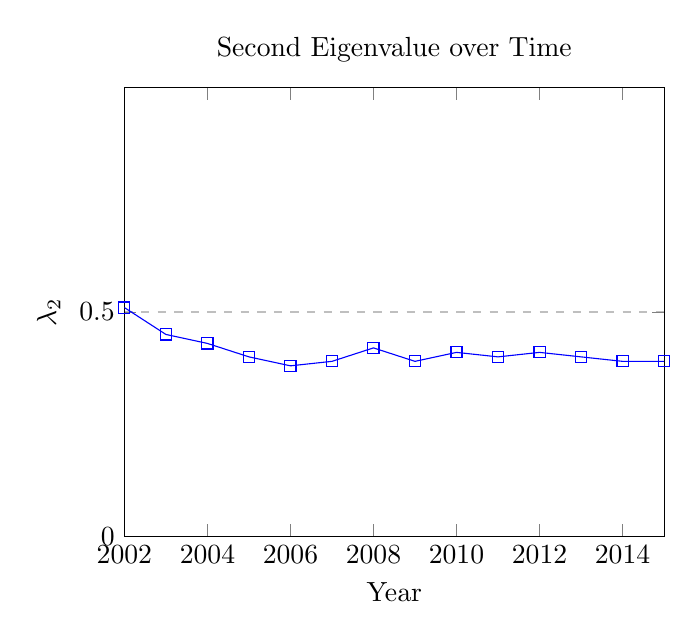
\begin{tikzpicture}
\begin{axis}[
    title={Second Eigenvalue over Time},
    xlabel={Year},
    ylabel={$\lambda_2$},
    xmin=2002, xmax=2015,
    ymin=0, ymax=1,
    xtick={2002, 2004, 2006, 2008, 2010, 2012, 2014},
    ytick={0, 0.5},
    legend pos=north west,
    ymajorgrids=true,
    grid style=dashed,
    tick label style={/pgf/number format/set thousands separator = {}}
]
 
\addplot[
    color=blue,
    mark=square,
    ]
    coordinates {
    (2002, 0.51)
    (2003, 0.45)
    (2004, 0.43)
    (2005, 0.40)
    (2006, 0.38)
    (2007, 0.39)
    (2008, 0.42)
    (2009, 0.39)
    (2010, 0.41)
    (2011, 0.40)
    (2012, 0.41)
    (2013, 0.40)
    (2014, 0.39)
    (2015, 0.39)
    };

\end{axis}
\end{tikzpicture}
\end{center}

Next I will take a look at how the different neighborhoods specialize in different job industries.  The eigenvector centrality is able to pull out the different networks of employment in Chicago such as how dispersed the Goods Producing sector is compared to the Trade, Transportation, and Utilities sector which is dominated by O'Hare International Airport.  The Other category is dominated by The Loop area where most of the jobs in the city are located. \\

\begin{figure}[H]
    \centering
    \includegraphics[width=0.31\textwidth]{Jobs-SI001-2015}
    \includegraphics[width=0.31\textwidth]{Jobs-SI002-2015}
    \includegraphics[width=0.31\textwidth]{Jobs-SI003-2015}
    \caption{2015 eigenvectors for the three different industry categories: Goods Producing (left), Trade, Transportation, Utilities (center), Other (right)}
    \label{fig:Jobs-S000-2008}
\end{figure}

Lastly I will look at the eigenvectors across different income levels.  What is interesting about these graphs is how similar the principal eigenvectors are be by income levels.  Even though parts of Chicago are segregated by income level, the importance of each neighborhood for jobs is very similar.

\begin{figure}[H]
    \centering
    \includegraphics[width=0.31\textwidth]{Jobs-SE001-2015}
    \includegraphics[width=0.31\textwidth]{Jobs-SE002-2015}
    \includegraphics[width=0.31\textwidth]{Jobs-SE003-2015}
    \caption{2015 eigenvectors for the three different salary levels: Under \$1,250 left, \$1,250 - \$3,333 center, Over \$3,333 right for 2015.}
    \label{fig:Jobs-S000-2008}
\end{figure}

Above I used the theory of eigenvector centrality to rank the most important neighborhoods of employment for neighborhoods in Chicago.  This perspective gives us a rich view of the composition of a neighborhood as well as how it changes over time in comparison to other neighborhoods in the city.

\subsection{Centrality for Housing}
Similar to how employment centrality was calculated, I calculate housing centrality, answering the question \textit{What neighborhoods are the most important for housing}?  I also break down the neighborhood centrality by most important for High and Low income earners and Old age and Young age based off of the LEHD Dataset.  Below I map the principal eigenvector across the whole population in 2015.  From this map it is apparent the network structure for housing is a lot different than for employment. The distributions of the rankings are a lot more even across neighborhoods compared to the employment dataset which was dominated by The Loop neighborhood.  The top 10 neighborhoods based on their centrality from 2015 are listed below.  The rankings are much more stable over time than they were for the employment dataset as most neighborhoods only increasing or decreasing in the single digits over the 14 year timespan.\footnote{Graphs for this section are also included in the Appendix.}\\

{\centering
\begin{figure}[H]
    \centering
    \includegraphics[width=0.75\textwidth]{Houses-S000-2015}
    \caption{This map shows the eigenvector that corresponds to the principal eigenvalue in 2015.}
    \label{fig:Houses-S000-2015}
\end{figure} } \\


\begin{table}[h]\centering
\caption{Overall Housing Rank}\label{thelabel}

\begin{adjustbox}{center}
\begin{tabular}{||c | c c c c c c c c c c c c c c | c ||} 
 \hline
 & 2002 & 2003 & 2004 & 2005 & 2006 & 2007 & 2008 & 2009 & 2010 & 2011 & 2012 & 2013 & 2014 & 2015 & | \%\\[0.5ex] 
 \hline\hline
Logan Square & .303 & .307 & .307 & .296 & .287 & .207 & .296 & .201 & .313 & .316 & .323 & .333 & .340 & .322 & 6.27\% \\
West Rogers Park & .220 & .221 & .221 & .224 & .230 & .201 & .221 & .209 & .246 & .260 & .261 & .254 & .245 & .239 & 8.64\% \\
Gresham & .238 & .239 & .239 & .233 & .231 & .245 & .242 & .254 & .202 & .205 & .213 & .193 & .201 & .215 & -9.66\% \\
Portage Park & .188 & .185 & .185 & .181 & .182 & .214 & .191 & .220 & .201 & .203 & .190 & .198 & .188 & .189 & .53\% \\
Archer Heights & .181 & .178 & .178 & .186 & .182 & .187 & .173 & .185 & .198 & .173 & .175 & .184 & .186 & .188 & 3.87\% \\
Little Village & .208 & .200 & .200 & .196 & .193 & .201 & .176 & .201 & .178 & .171 & .183 & .187 & .197 & .188 & -9.62\% \\
Albany Park & .189 & .195 & .195 & .179 & .172 & .144 & .181 & .133 & .186 & .198 & .201 & .193 & .183 & .179 & -5.29\% \\
Englewood & .247 & .244 & .244 & .236 & .239 & .258 & .223 & .252 & .197 & .185 & .178 & .172 & .177 & .179 & -27.53\% \\
Bridgeport & .139 & .147 & .147 & .146 & .157 & .171 & .165 & .181 & .189 & .171 & .176 & .175 & .171 & .174 & 25.18\% \\
Rogers Park & .154 & .151 & .151 & .150 & .159 & .133 & .155 & .127 & .158 & .172 & .175 & .177 & .175 & .174 & 12.99\% \\ \hline
 \end{tabular}
\end{adjustbox}
\end{table}


fAfter the centrality measurements are created we can start to ask interesting questions such as how neighborhoods are changing overtime in comparison to each other.  The main dimensions I will look at are how the age and income are affecting neighborhoods in Chicago.  Below are tables of the top 10 neighborhoods by centrality ranking for Young/Old workers and Low-Income/High Income workers.\\

\begin{table}[h]\centering
\caption{Housing Rank - Age $<$ 29}\label{thelabel}
\begin{adjustbox}{center}
\begin{tabular}{||c | c c c c c c c c c c c c c c | c ||} 
 \hline
 & 2002 & 2003 & 2004 & 2005 & 2006 & 2007 & 2008 & 2009 & 2010 & 2011 & 2012 & 2013 & 2014 & 2015 & | \%\\[0.5ex] 
 \hline\hline
Logan Square & .355 & .364 & .341 & .353 & .338 & .262 & .368 & .235 & .388 & .385 & .398 & .408 & .391 & .385 & 8.45\% \\
Little Village & .248 & .247 & .244 & .253 & .234 & .235 & .200 & .228 & .207 & .202 & .224 & .224 & .230 & .217 & -12.50\% \\
Gresham & .194 & .201 & .215 & .197 & .190 & .209 & .219 & .227 & .164 & .173 & .174 & .158 & .187 & .209 & 7.73\% \\
Englewood & .244 & .257 & .253 & .239 & .234 & .262 & .226 & .254 & .183 & .157 & .165 & .162 & .175 & .205 & -15.98\% \\
Archer Heights & .197 & .184 & .191 & .199 & .191 & .198 & .174 & .205 & .209 & .166 & .186 & .195 & .198 & .189 & -4.06\% \\
Lake View & .155 & .171 & .191 & .185 & .212 & .186 & .214 & .156 & .240 & .215 & .208 & .191 & .177 & .187 & 2.65\% \\
Brighton Park & .187 & .189 & .182 & .186 & .189 & .145 & .158 & .145 & .156 & .164 & .159 & .183 & .170 & .179 & -4.28\% \\
West Rogers Park & .169 & .165 & .168 & .176 & .169 & .169 & .178 & .185 & .192 & .206 & .208 & .191 & .175 & .178 & 5.33\% \\
Rogers Park & .142 & .139 & .140 & .144 & .153 & .126 & .145 & .135 & .154 & .166 & .154 & .154 & .158 & .174 & 22.54\% \\
Marquette Park & .140 & .144 & .150 & .176 & .180 & .164 & .151 & .160 & .131 & .132 & .135 & .124 & .142 & .167 & 19.29\% \\
 \hline
 \end{tabular}

\end{adjustbox}
 \end{table}
 
\begin{table}[h]\centering
\caption{Housing Rank - Age over 55}\label{thelabel}
\begin{adjustbox}{center}
\begin{tabular}{||c | c c c c c c c c c c c c c c | c ||} 
 \hline
 & 2002 & 2003 & 2004 & 2005 & 2006 & 2007 & 2008 & 2009 & 2010 & 2011 & 2012 & 2013 & 2014 & 2015 & | \%\\[0.5ex] 
 \hline\hline
West Rogers Park & .229 & .248 & .234 & .220 & .225 & .186 & .247 & .183 & .273 & .293 & .301 & .302 & .273 & .281 & 22.71\% \\
Logan Square & .231 & .224 & .223 & .201 & .211 & .129 & .196 & .167 & .234 & .225 & .240 & .246 & .265 & .239 & 3.46\% \\
Portage Park & .183 & .202 & .213 & .204 & .189 & .220 & .219 & .239 & .216 & .240 & .225 & .215 & .242 & .235 & 28.42\% \\
Gresham & .314 & .292 & .319 & .312 & .301 & .280 & .261 & .283 & .238 & .238 & .221 & .220 & .228 & .229 & -27.07\% \\
Jefferson Park & .193 & .200 & .185 & .194 & .184 & .189 & .225 & .194 & .231 & .208 & .204 & .214 & .235 & .208 & 7.77\% \\
Bridgeport & .119 & .139 & .148 & .134 & .151 & .189 & .170 & .190 & .200 & .185 & .191 & .209 & .197 & .194 & 63.03\% \\
Albany Park & .155 & .164 & .159 & .164 & .150 & .118 & .176 & .121 & .174 & .179 & .192 & .182 & .175 & .186 & 2.00\% \\
Archer Heights & .159 & .156 & .155 & .181 & .173 & .178 & .168 & .167 & .194 & .160 & .163 & .172 & .158 & .168 & 5.66\% \\
Little Village & .150 & .154 & .164 & .162 & .169 & .181 & .150 & .196 & .155 & .145 & .167 & .163 & .171 & .161 & 7.33\% \\
West Pullman & .185 & .205 & .189 & .177 & .241 & .172 & .175 & .179 & .164 & .153 & .142 & .138 & .142 & .161 & -12.97\% \\
 \hline
 \end{tabular}

\end{adjustbox}
\end{table}

\begin{table}[h]\centering
\caption{Housing Rank -  Income $<$ \$1,250/month}\label{thelabel}
\begin{adjustbox}{center}
\begin{tabular}{||c | c c c c c c c c c c c c c c | c ||} 
 \hline
 & 2002 & 2003 & 2004 & 2005 & 2006 & 2007 & 2008 & 2009 & 2010 & 2011 & 2012 & 2013 & 2014 & 2015 & | \%\\[0.5ex] 
 \hline\hline
Gresham & .254 & .259 & .259 & .256 & .263 & .247 & .278 & .287 & .237 & .234 & .240 & .220 & .255 & .280 & 1.24\% \\
Englewood & .310 & .296 & .296 & .290 & .314 & .325 & .292 & .299 & .245 & .223 & .227 & .222 & .257 & .271 & -12.58\% \\
Logan Square & .272 & .283 & .283 & .262 & .247 & .183 & .255 & .194 & .293 & .286 & .284 & .304 & .280 & .246 & -9.56\% \\
West Rogers Park & .201 & .224 & .224 & .232 & .222 & .190 & .220 & .195 & .249 & .272 & .240 & .248 & .220 & .218 & 8.46\% \\
Archer Heights & .189 & .204 & .204 & .195 & .182 & .191 & .187 & .181 & .198 & .190 & .192 & .207 & .204 & .211 & 11.64\% \\
Bridgeport & .158 & .185 & .185 & .182 & .195 & .196 & .191 & .206 & .217 & .196 & .207 & .197 & .186 & .190 & 2.25\% \\
Little Village & .212 & .208 & .208 & .199 & .200 & .201 & .180 & .184 & .172 & .164 & .192 & .206 & .199 & .183 & -13.68\% \\
West Pullman & .196 & .180 & .180 & .153 & .174 & .142 & .170 & .171 & .172 & .137 & .173 & .151 & .173 & .177 & -9.69\% \\
South Shore & .172 & .153 & .153 & .166 & .174 & .184 & .190 & .203 & .144 & .161 & .155 & .152 & .158 & .176 & 2.33\% \\
Back of the Yards & .183 & .172 & .172 & .185 & .188 & .164 & .182 & .164 & .194 & .171 & .169 & .171 & .166 & .172 & -6.01\% \\
\hline
 \end{tabular}
\end{adjustbox}
\end{table}


\begin{table}[h]\centering
\caption{Housing Rank - Income $>$ \$3,333/month}\label{thelabel}
\begin{adjustbox}{center}
\begin{tabular}{||c | c c c c c c c c c c c c c c | c ||} 
 \hline
 & 2002 & 2003 & 2004 & 2005 & 2006 & 2007 & 2008 & 2009 & 2010 & 2011 & 2012 & 2013 & 2014 & 2015 & | \%\\[0.5ex] 
 \hline\hline
Logan Square & .235 & .261 & .249 & .240 & .262 & .198 & .282 & .221 & .295 & .305 & .300 & .331 & .350 & .335 & 42.55\% \\
Lake View & .331 & .342 & .307 & .332 & .331 & .263 & .319 & .289 & .345 & .323 & .359 & .330 & .312 & .321 & -3.02\% \\
West Rogers Park & .291 & .273 & .293 & .272 & .290 & .262 & .268 & .302 & .284 & .281 & .270 & .265 & .266 & .264 & -9.28\% \\
Lake View East & .241 & .257 & .243 & .278 & .279 & .202 & .262 & .185 & .233 & .239 & .241 & .237 & .242 & .243 & .83\% \\
Jefferson Park & .248 & .257 & .267 & .246 & .235 & .251 & .259 & .237 & .207 & .214 & .228 & .237 & .247 & .226 & -8.87\% \\
Portage Park & .239 & .216 & .203 & .196 & .195 & .226 & .194 & .212 & .186 & .190 & .189 & .191 & .183 & .202 & -15.48\% \\
Albany Park & .159 & .161 & .166 & .171 & .164 & .159 & .186 & .138 & .178 & .204 & .205 & .204 & .190 & .191 & 2.13\% \\
Rogers Park & .166 & .174 & .167 & .180 & .186 & .165 & .181 & .157 & .191 & .190 & .191 & .188 & .175 & .187 & 12.65\% \\
Ravenswood & .169 & .171 & .164 & .157 & .166 & .145 & .175 & .150 & .187 & .190 & .174 & .170 & .172 & .187 & 1.65\% \\ \end{tabular}
\end{adjustbox}
\end{table}

Above we can notice a few interesting trends, for example, some neighborhoods becoming a lot more influential for young workers such as Lake View, Rogers Park, and Marquette Park while others becoming more influential for older workers such as West Rogers Park, Portage Park, Bridgeport, and Albany Park. \\

There has also have been some larger shifts in where low income workers are moving such as moving into Gresham and Bridgeport whereas High Income earners have been flocking to Logan Square, Albany Park, and especially the South Loop whose importance has risen 66\% since 2002. \\

Another interesting statistic we can calculate from using the eigenvector centrality scores is how neighborhood composition is changing.  For example, while previously I just calculated ranking along one demographic indicator I can combine rankings to describe neighborhoods in new ways.  One way to do this is by subtracting the neighborhood ranking of young and old workers or high income and low income workers.  This could help detect neighborhood changes such as gentrification or income changes and potentially produce different rankings than if neighborhoods were scored according to a single demographic indicator.  For example, it could be that a neighborhood is becoming a higher rank for both young and old workers.  This would most likely be a different kind of neighborhood change than a neighborhood that becomes a higher rank for young workers and a lower rank for old workers.  Below I calculate this metric by subtracting the trend lines of rankings between these two eigenvectors. \\

\begin{table}[!htb]

\caption{Housing Rank Income Changes}\label{thelabel}
\begin{minipage}{.5\linewidth}
      \caption{Low to High}
      \centering
      
\begin{tabular}{||c | c ||} 
 \hline
Neighborhood &  \%\\[0.5ex] 
 \hline\hline
Bridgeport & 0.456 \\
Portage Park & 0.386 \\
West Rogers Park & 0.384 \\
Brighton Park & 0.356 \\
West Lawn & 0.329 \\
Albany Park & 0.325 \\
Little Village & 0.306 \\
Gage Park & 0.261 \\
Back of the Yards & 0.219 \\
Jefferson Park & 0.208 \\
\hline
 \end{tabular}

\end{minipage}%
    \begin{minipage}{.5\linewidth}
      \centering
\caption{High to Low}\label{thelabel}

\begin{tabular}{||c | c ||} 
 \hline
Neighborhood &  \%\\[0.5ex] 
 \hline\hline
Gresham & 0.640 \\
Calumet Heights & 0.437 \\
Fernwood & 0.409 \\
Roseland & 0.390 \\
West Pullman & 0.334 \\
West Englewood & 0.327 \\
Chatham & 0.324 \\
Morgan Park & 0.298 \\
Rosemoor & 0.294 \\
Hegewisch & 0.271 \\
\hline
\end{tabular}
\end{minipage} 
\end{table}

\begin{table}[!htb]

\caption{Housing Rank Income Changes}\label{thelabel}
\begin{minipage}{.5\linewidth}
      \caption{Low to High}
      \centering
      
\begin{tabular}{||c | c ||} 
 \hline
Neighborhood &  Rank\\[0.5ex] 
 \hline\hline
Marquette Park & 0.423 \\
Jefferson Park & 0.420 \\
Portage Park & 0.405 \\
Morgan Park & 0.365 \\
Beverly & 0.343 \\
West Lawn & 0.328 \\
West Rogers Park & 0.327 \\
East Side & 0.292 \\
Wrightwood & 0.261 \\
Garfield Ridge & 0.254 \\
\hline
 \end{tabular}

\end{minipage}%
    \begin{minipage}{.5\linewidth}
      \centering
\caption{High to Low}\label{thelabel}

\begin{tabular}{||c | c ||} 
 \hline
Neighborhood &  Rank\\[0.5ex] 
 \hline\hline
Logan Square & 0.757 \\
Albany Park & 0.492 \\
South Loop & 0.329 \\
Humboldt Park & 0.311 \\
Ravenswood & 0.227 \\
Englewood & 0.196 \\
West Town & 0.177 \\
Heart of Chicago & 0.176 \\
The Loop & 0.170 \\
East Ukrainian Village & 0.157 \\
\hline
 \end{tabular}
\end{minipage} 
\end{table}

\\

Though I have shown that much can be learned about a neighborhood by its eigenvector centrality.  The neighborhood rankings produced are potentially hard to interpret and analyze.  For example, while we know that a neighborhood ranks high for an age group and income level, what else does this ranking tell us about a city.  To analyze this I will look how centrality rankings correspond to other attributes about a neighborhood first by looking at correlation to housing stock and value.

\begin{comment}
\subsection{To Do: Centrality for Money Flow}
I am currently working on the computation for this section.  The idea is outlined in the methods section where I will calculate neighborhood importance based off of the money that flow between neighborhoods (this is based on salary * number of workers).  I will also add outside data from construction permits etc to help with this analysis.\cite{gould1967geographical}
\end{comment}

\section{Conclusion}
In this paper I presented a novel application of eigenvector centrality to dataset of Chicago's neighborhoods.  After exploring the data through visualizations, I derived the math necessary for this application and outlined three examples where eigenvector centrality can help explore attributes of Chicago neighborhoods.  First, I looked at how jobs were distributed across the city.  In this analysis I found how employment was centralized in the Loop.  While jobs in some industries such as Goods Producing are also located a west of downtown, The Loop neighborhood ranked at .95 while the next closest neighborhood ranked .17.  Even low-income jobs were concentrated in The Loop which was surprising.  While The Loop was a mixing pot of employment across industries, incomes, and ages, Housing centrality was much more segregated and dispersed throughout the city.  For example, I found that 

\section{Appendix}

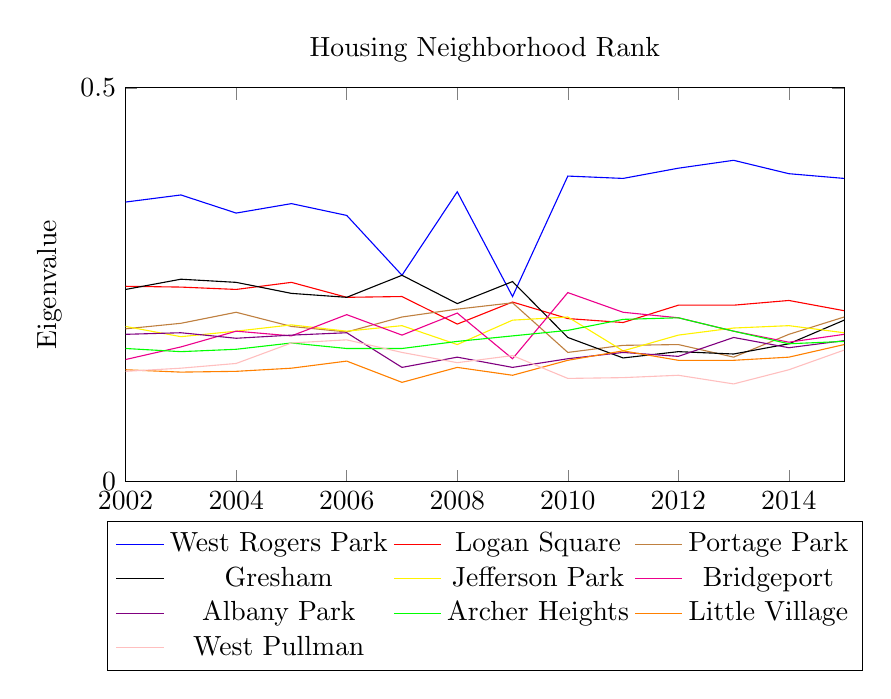
\begin{tikzpicture}
\begin{axis}[
    title={Housing Neighborhood Rank},
    xlabel={Year},
    ylabel={Eigenvalue},
    xmin=2002, 
    xmax=2015,
    ymin=0, 
    ymax=0.5,
    clip bounding box=upper bound,
    ylabel near ticks,
    scale only axis, 
    width=\textwidth - 3cm,
    height=5cm,
    xtick={2002, 2004, 2006, 2008, 2010, 2012, 2014},
    ytick={0, 0.5},
    legend columns=3,
    legend style={at={(0.5,-0.1)},anchor=north},
    ymajorgrids=true,
    grid style=dashed,
    tick label style={/pgf/number format/set thousands separator = {}}
]
 

\addplot[color=blue] coordinates {(2002, 0.355)  (2003, 0.364)  (2004, 0.341)  (2005, 0.353)  (2006, 0.338)  (2007, 0.262)  (2008, 0.368)  (2009, 0.235)  (2010, 0.388)  (2011, 0.385)  (2012, 0.398)  (2013, 0.408)  (2014, 0.391)  (2015, 0.385)};

\addplot[color=red] coordinates {(2002, 0.248)  (2003, 0.247)  (2004, 0.244)  (2005, 0.253)  (2006, 0.234)  (2007, 0.235)  (2008, 0.2)  (2009, 0.228)  (2010, 0.207)  (2011, 0.202)  (2012, 0.224)  (2013, 0.224)  (2014, 0.23)  (2015, 0.217)};

\addplot[color=brown] coordinates {(2002, 0.194)  (2003, 0.201)  (2004, 0.215)  (2005, 0.197)  (2006, 0.19)  (2007, 0.209)  (2008, 0.219)  (2009, 0.227)  (2010, 0.164)  (2011, 0.173)  (2012, 0.174)  (2013, 0.158)  (2014, 0.187)  (2015, 0.209)};

\addplot[color=black] coordinates {(2002, 0.244)  (2003, 0.257)  (2004, 0.253)  (2005, 0.239)  (2006, 0.234)  (2007, 0.262)  (2008, 0.226)  (2009, 0.254)  (2010, 0.183)  (2011, 0.157)  (2012, 0.165)  (2013, 0.162)  (2014, 0.175)  (2015, 0.205)};

\addplot[color=yellow] coordinates {(2002, 0.197)  (2003, 0.184)  (2004, 0.191)  (2005, 0.199)  (2006, 0.191)  (2007, 0.198)  (2008, 0.174)  (2009, 0.205)  (2010, 0.209)  (2011, 0.166)  (2012, 0.186)  (2013, 0.195)  (2014, 0.198)  (2015, 0.189)};

\addplot[color=magenta] coordinates {(2002, 0.155)  (2003, 0.171)  (2004, 0.191)  (2005, 0.185)  (2006, 0.212)  (2007, 0.186)  (2008, 0.214)  (2009, 0.156)  (2010, 0.24)  (2011, 0.215)  (2012, 0.208)  (2013, 0.191)  (2014, 0.177)  (2015, 0.187)};

\addplot[color=violet] coordinates {(2002, 0.187)  (2003, 0.189)  (2004, 0.182)  (2005, 0.186)  (2006, 0.189)  (2007, 0.145)  (2008, 0.158)  (2009, 0.145)  (2010, 0.156)  (2011, 0.164)  (2012, 0.159)  (2013, 0.183)  (2014, 0.17)  (2015, 0.179)};

\addplot[color=green] coordinates {(2002, 0.169)  (2003, 0.165)  (2004, 0.168)  (2005, 0.176)  (2006, 0.169)  (2007, 0.169)  (2008, 0.178)  (2009, 0.185)  (2010, 0.192)  (2011, 0.206)  (2012, 0.208)  (2013, 0.191)  (2014, 0.175)  (2015, 0.178)};

\addplot[color=orange] coordinates {(2002, 0.142)  (2003, 0.139)  (2004, 0.14)  (2005, 0.144)  (2006, 0.153)  (2007, 0.126)  (2008, 0.145)  (2009, 0.135)  (2010, 0.154)  (2011, 0.166)  (2012, 0.154)  (2013, 0.154)  (2014, 0.158)  (2015, 0.174)};

\addplot[color=pink] coordinates {(2002, 0.14)  (2003, 0.144)  (2004, 0.15)  (2005, 0.176)  (2006, 0.18)  (2007, 0.164)  (2008, 0.151)  (2009, 0.16)  (2010, 0.131)  (2011, 0.132)  (2012, 0.135)  (2013, 0.124)  (2014, 0.142)  (2015, 0.167)};
\legend{West Rogers Park,Logan Square,Portage Park,Gresham,Jefferson Park,Bridgeport,Albany Park,Archer Heights,Little Village,West Pullman}

\end{axis}
\end{tikzpicture}

\vspace{2cm} \\

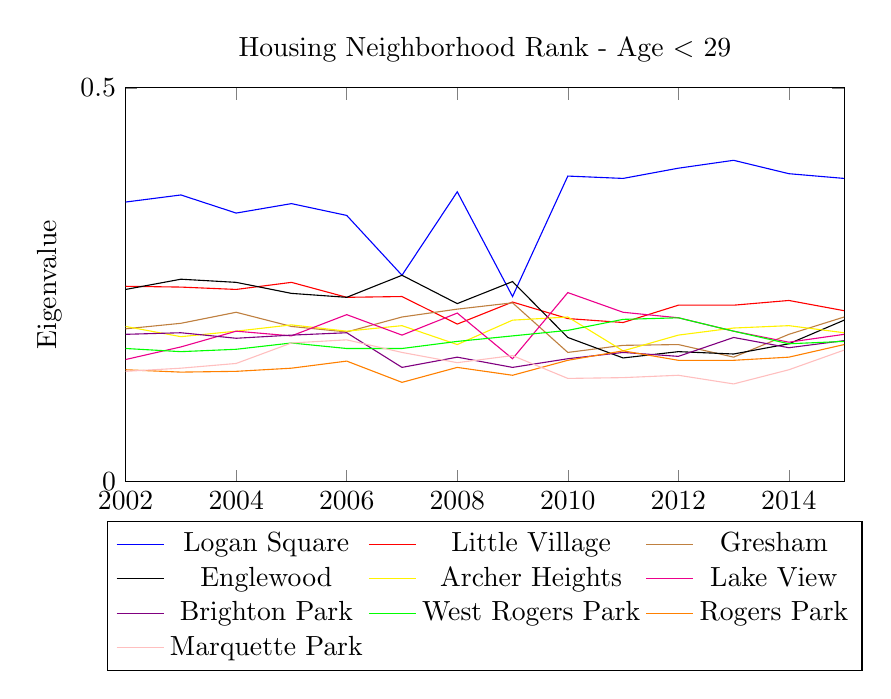
\begin{tikzpicture}
\begin{axis}[
    title={Housing Neighborhood Rank - Age $<$ 29},
    xlabel={Year},
    ylabel={Eigenvalue},
    xmin=2002, 
    xmax=2015,
    ymin=0, 
    ymax=0.5,
    clip bounding box=upper bound,
    ylabel near ticks,
    scale only axis, 
    width=\textwidth - 3cm,
    height=5cm,
    xtick={2002, 2004, 2006, 2008, 2010, 2012, 2014},
    ytick={0, 0.5},
    legend columns=3,
    legend style={at={(0.5,-0.1)},anchor=north},
    ymajorgrids=true,
    grid style=dashed,
    tick label style={/pgf/number format/set thousands separator = {}}
]
 

\addplot[color=blue] coordinates {(2002, 0.355)  (2003, 0.364)  (2004, 0.341)  (2005, 0.353)  (2006, 0.338)  (2007, 0.262)  (2008, 0.368)  (2009, 0.235)  (2010, 0.388)  (2011, 0.385)  (2012, 0.398)  (2013, 0.408)  (2014, 0.391)  (2015, 0.385)};

\addplot[color=red] coordinates {(2002, 0.248)  (2003, 0.247)  (2004, 0.244)  (2005, 0.253)  (2006, 0.234)  (2007, 0.235)  (2008, 0.2)  (2009, 0.228)  (2010, 0.207)  (2011, 0.202)  (2012, 0.224)  (2013, 0.224)  (2014, 0.23)  (2015, 0.217)};

\addplot[color=brown] coordinates {(2002, 0.194)  (2003, 0.201)  (2004, 0.215)  (2005, 0.197)  (2006, 0.19)  (2007, 0.209)  (2008, 0.219)  (2009, 0.227)  (2010, 0.164)  (2011, 0.173)  (2012, 0.174)  (2013, 0.158)  (2014, 0.187)  (2015, 0.209)};

\addplot[color=black] coordinates {(2002, 0.244)  (2003, 0.257)  (2004, 0.253)  (2005, 0.239)  (2006, 0.234)  (2007, 0.262)  (2008, 0.226)  (2009, 0.254)  (2010, 0.183)  (2011, 0.157)  (2012, 0.165)  (2013, 0.162)  (2014, 0.175)  (2015, 0.205)};

\addplot[color=yellow] coordinates {(2002, 0.197)  (2003, 0.184)  (2004, 0.191)  (2005, 0.199)  (2006, 0.191)  (2007, 0.198)  (2008, 0.174)  (2009, 0.205)  (2010, 0.209)  (2011, 0.166)  (2012, 0.186)  (2013, 0.195)  (2014, 0.198)  (2015, 0.189)};

\addplot[color=magenta] coordinates {(2002, 0.155)  (2003, 0.171)  (2004, 0.191)  (2005, 0.185)  (2006, 0.212)  (2007, 0.186)  (2008, 0.214)  (2009, 0.156)  (2010, 0.24)  (2011, 0.215)  (2012, 0.208)  (2013, 0.191)  (2014, 0.177)  (2015, 0.187)};

\addplot[color=violet] coordinates {(2002, 0.187)  (2003, 0.189)  (2004, 0.182)  (2005, 0.186)  (2006, 0.189)  (2007, 0.145)  (2008, 0.158)  (2009, 0.145)  (2010, 0.156)  (2011, 0.164)  (2012, 0.159)  (2013, 0.183)  (2014, 0.17)  (2015, 0.179)};

\addplot[color=green] coordinates {(2002, 0.169)  (2003, 0.165)  (2004, 0.168)  (2005, 0.176)  (2006, 0.169)  (2007, 0.169)  (2008, 0.178)  (2009, 0.185)  (2010, 0.192)  (2011, 0.206)  (2012, 0.208)  (2013, 0.191)  (2014, 0.175)  (2015, 0.178)};

\addplot[color=orange] coordinates {(2002, 0.142)  (2003, 0.139)  (2004, 0.14)  (2005, 0.144)  (2006, 0.153)  (2007, 0.126)  (2008, 0.145)  (2009, 0.135)  (2010, 0.154)  (2011, 0.166)  (2012, 0.154)  (2013, 0.154)  (2014, 0.158)  (2015, 0.174)};

\addplot[color=pink] coordinates {(2002, 0.14)  (2003, 0.144)  (2004, 0.15)  (2005, 0.176)  (2006, 0.18)  (2007, 0.164)  (2008, 0.151)  (2009, 0.16)  (2010, 0.131)  (2011, 0.132)  (2012, 0.135)  (2013, 0.124)  (2014, 0.142)  (2015, 0.167)};
\legend{Logan Square,Little Village,Gresham,Englewood,Archer Heights,Lake View,Brighton Park,West Rogers Park,Rogers Park,Marquette Park}

\end{axis}
\end{tikzpicture}

\vspace{2cm} \\

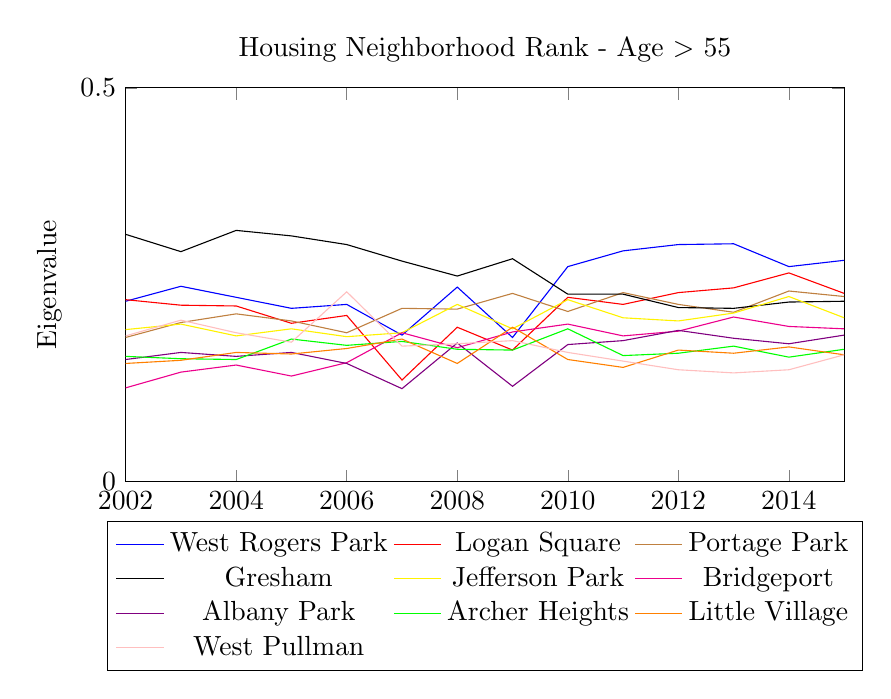
\begin{tikzpicture}
\begin{axis}[
    title={Housing Neighborhood Rank - Age $>$ 55},
    xlabel={Year},
    ylabel={Eigenvalue},
    xmin=2002, 
    xmax=2015,
    ymin=0, 
    ymax=0.5,
    clip bounding box=upper bound,
    ylabel near ticks,
    scale only axis, 
    width=\textwidth - 3cm,
    height=5cm,
    xtick={2002, 2004, 2006, 2008, 2010, 2012, 2014},
    ytick={0, 0.5},
    legend columns=3,
    legend style={at={(0.5,-0.1)},anchor=north},
    ymajorgrids=true,
    grid style=dashed,
    tick label style={/pgf/number format/set thousands separator = {}}
]
 

\addplot[color=blue] coordinates {(2002, 0.229)  (2003, 0.248)  (2004, 0.234)  (2005, 0.22)  (2006, 0.225)  (2007, 0.186)  (2008, 0.247)  (2009, 0.183)  (2010, 0.273)  (2011, 0.293)  (2012, 0.301)  (2013, 0.302)  (2014, 0.273)  (2015, 0.281)};

\addplot[color=red] coordinates {(2002, 0.231)  (2003, 0.224)  (2004, 0.223)  (2005, 0.201)  (2006, 0.211)  (2007, 0.129)  (2008, 0.196)  (2009, 0.167)  (2010, 0.234)  (2011, 0.225)  (2012, 0.24)  (2013, 0.246)  (2014, 0.265)  (2015, 0.239)};

\addplot[color=brown] coordinates {(2002, 0.183)  (2003, 0.202)  (2004, 0.213)  (2005, 0.204)  (2006, 0.189)  (2007, 0.22)  (2008, 0.219)  (2009, 0.239)  (2010, 0.216)  (2011, 0.24)  (2012, 0.225)  (2013, 0.215)  (2014, 0.242)  (2015, 0.235)};

\addplot[color=black] coordinates {(2002, 0.314)  (2003, 0.292)  (2004, 0.319)  (2005, 0.312)  (2006, 0.301)  (2007, 0.28)  (2008, 0.261)  (2009, 0.283)  (2010, 0.238)  (2011, 0.238)  (2012, 0.221)  (2013, 0.22)  (2014, 0.228)  (2015, 0.229)};

\addplot[color=yellow] coordinates {(2002, 0.193)  (2003, 0.2)  (2004, 0.185)  (2005, 0.194)  (2006, 0.184)  (2007, 0.189)  (2008, 0.225)  (2009, 0.194)  (2010, 0.231)  (2011, 0.208)  (2012, 0.204)  (2013, 0.214)  (2014, 0.235)  (2015, 0.208)};

\addplot[color=magenta] coordinates {(2002, 0.119)  (2003, 0.139)  (2004, 0.148)  (2005, 0.134)  (2006, 0.151)  (2007, 0.189)  (2008, 0.17)  (2009, 0.19)  (2010, 0.2)  (2011, 0.185)  (2012, 0.191)  (2013, 0.209)  (2014, 0.197)  (2015, 0.194)};

\addplot[color=violet] coordinates {(2002, 0.155)  (2003, 0.164)  (2004, 0.159)  (2005, 0.164)  (2006, 0.15)  (2007, 0.118)  (2008, 0.176)  (2009, 0.121)  (2010, 0.174)  (2011, 0.179)  (2012, 0.192)  (2013, 0.182)  (2014, 0.175)  (2015, 0.186)};

\addplot[color=green] coordinates {(2002, 0.159)  (2003, 0.156)  (2004, 0.155)  (2005, 0.181)  (2006, 0.173)  (2007, 0.178)  (2008, 0.168)  (2009, 0.167)  (2010, 0.194)  (2011, 0.16)  (2012, 0.163)  (2013, 0.172)  (2014, 0.158)  (2015, 0.168)};

\addplot[color=orange] coordinates {(2002, 0.15)  (2003, 0.154)  (2004, 0.164)  (2005, 0.162)  (2006, 0.169)  (2007, 0.181)  (2008, 0.15)  (2009, 0.196)  (2010, 0.155)  (2011, 0.145)  (2012, 0.167)  (2013, 0.163)  (2014, 0.171)  (2015, 0.161)};

\addplot[color=pink] coordinates {(2002, 0.185)  (2003, 0.205)  (2004, 0.189)  (2005, 0.177)  (2006, 0.241)  (2007, 0.172)  (2008, 0.175)  (2009, 0.179)  (2010, 0.164)  (2011, 0.153)  (2012, 0.142)  (2013, 0.138)  (2014, 0.142)  (2015, 0.161)};
\legend{West Rogers Park,Logan Square,Portage Park,Gresham,Jefferson Park,Bridgeport,Albany Park,Archer Heights,Little Village,West Pullman}

\end{axis}
\end{tikzpicture}

\vspace{2cm} \\

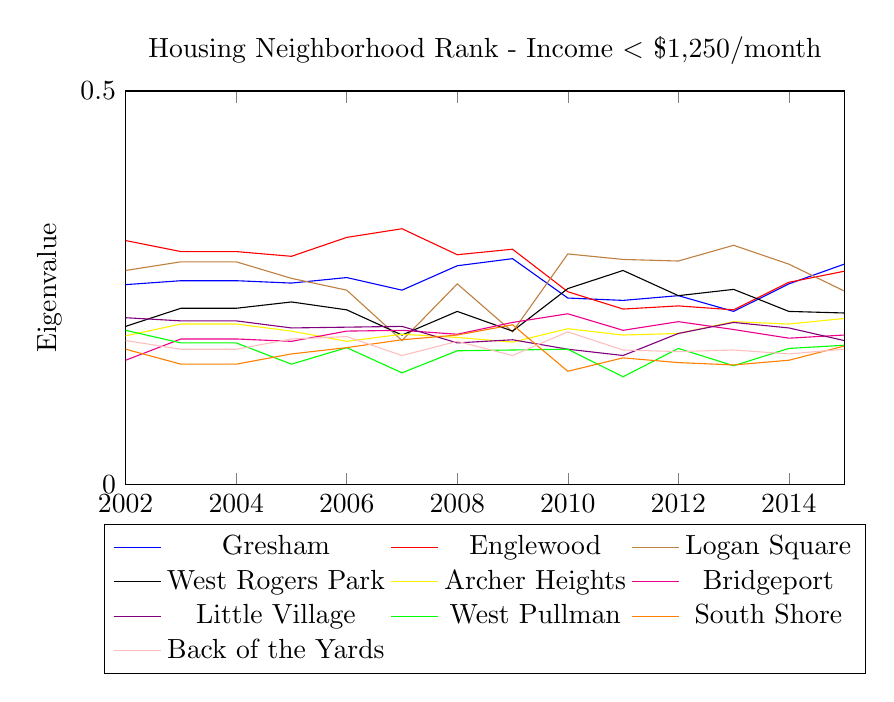
\begin{tikzpicture}
\begin{axis}[
    title={Housing Neighborhood Rank - Income $<$ \$1,250/month},
    xlabel={Year},
    ylabel={Eigenvalue},
    xmin=2002, 
    xmax=2015,
    ymin=0, 
    ymax=0.5,
    clip bounding box=upper bound,
    ylabel near ticks,
    scale only axis, 
    width=\textwidth - 3cm,
    height=5cm,
    xtick={2002, 2004, 2006, 2008, 2010, 2012, 2014},
    ytick={0, 0.5},
    legend columns=3,
    legend style={at={(0.5,-0.1)},anchor=north},
    ymajorgrids=true,
    grid style=dashed,
    tick label style={/pgf/number format/set thousands separator = {}}
]
 

\addplot[color=blue] coordinates {(2002, 0.254)  (2003, 0.259)  (2004, 0.259)  (2005, 0.256)  (2006, 0.263)  (2007, 0.247)  (2008, 0.278)  (2009, 0.287)  (2010, 0.237)  (2011, 0.234)  (2012, 0.24)  (2013, 0.22)  (2014, 0.255)  (2015, 0.28)};

\addplot[color=red] coordinates {(2002, 0.31)  (2003, 0.296)  (2004, 0.296)  (2005, 0.29)  (2006, 0.314)  (2007, 0.325)  (2008, 0.292)  (2009, 0.299)  (2010, 0.245)  (2011, 0.223)  (2012, 0.227)  (2013, 0.222)  (2014, 0.257)  (2015, 0.271)};

\addplot[color=brown] coordinates {(2002, 0.272)  (2003, 0.283)  (2004, 0.283)  (2005, 0.262)  (2006, 0.247)  (2007, 0.183)  (2008, 0.255)  (2009, 0.194)  (2010, 0.293)  (2011, 0.286)  (2012, 0.284)  (2013, 0.304)  (2014, 0.28)  (2015, 0.246)};

\addplot[color=black] coordinates {(2002, 0.201)  (2003, 0.224)  (2004, 0.224)  (2005, 0.232)  (2006, 0.222)  (2007, 0.19)  (2008, 0.22)  (2009, 0.195)  (2010, 0.249)  (2011, 0.272)  (2012, 0.24)  (2013, 0.248)  (2014, 0.22)  (2015, 0.218)};

\addplot[color=yellow] coordinates {(2002, 0.189)  (2003, 0.204)  (2004, 0.204)  (2005, 0.195)  (2006, 0.182)  (2007, 0.191)  (2008, 0.187)  (2009, 0.181)  (2010, 0.198)  (2011, 0.19)  (2012, 0.192)  (2013, 0.207)  (2014, 0.204)  (2015, 0.211)};

\addplot[color=magenta] coordinates {(2002, 0.158)  (2003, 0.185)  (2004, 0.185)  (2005, 0.182)  (2006, 0.195)  (2007, 0.196)  (2008, 0.191)  (2009, 0.206)  (2010, 0.217)  (2011, 0.196)  (2012, 0.207)  (2013, 0.197)  (2014, 0.186)  (2015, 0.19)};

\addplot[color=violet] coordinates {(2002, 0.212)  (2003, 0.208)  (2004, 0.208)  (2005, 0.199)  (2006, 0.2)  (2007, 0.201)  (2008, 0.18)  (2009, 0.184)  (2010, 0.172)  (2011, 0.164)  (2012, 0.192)  (2013, 0.206)  (2014, 0.199)  (2015, 0.183)};

\addplot[color=green] coordinates {(2002, 0.196)  (2003, 0.18)  (2004, 0.18)  (2005, 0.153)  (2006, 0.174)  (2007, 0.142)  (2008, 0.17)  (2009, 0.171)  (2010, 0.172)  (2011, 0.137)  (2012, 0.173)  (2013, 0.151)  (2014, 0.173)  (2015, 0.177)};

\addplot[color=orange] coordinates {(2002, 0.172)  (2003, 0.153)  (2004, 0.153)  (2005, 0.166)  (2006, 0.174)  (2007, 0.184)  (2008, 0.19)  (2009, 0.203)  (2010, 0.144)  (2011, 0.161)  (2012, 0.155)  (2013, 0.152)  (2014, 0.158)  (2015, 0.176)};

\addplot[color=pink] coordinates {(2002, 0.183)  (2003, 0.172)  (2004, 0.172)  (2005, 0.185)  (2006, 0.188)  (2007, 0.164)  (2008, 0.182)  (2009, 0.164)  (2010, 0.194)  (2011, 0.171)  (2012, 0.169)  (2013, 0.171)  (2014, 0.166)  (2015, 0.172)};
\legend{Gresham,Englewood,Logan Square,West Rogers Park,Archer Heights,Bridgeport,Little Village,West Pullman,South Shore,Back of the Yards}

\end{axis}
\end{tikzpicture}

\vspace{2cm} \\

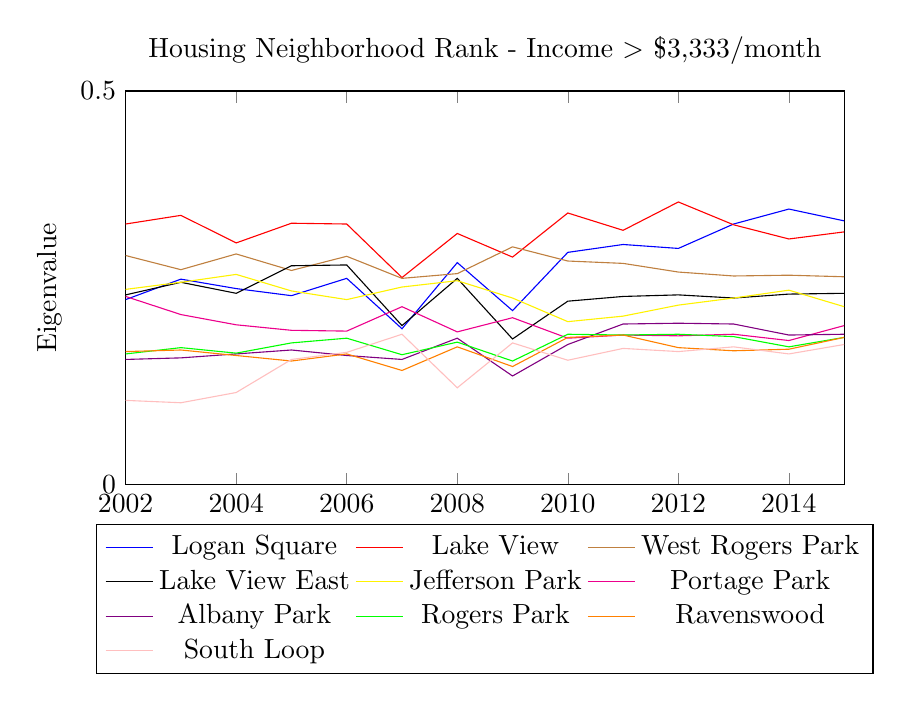
\begin{tikzpicture}
\begin{axis}[
    title={Housing Neighborhood Rank - Income $>$ \$3,333/month},
    xlabel={Year},
    ylabel={Eigenvalue},
    xmin=2002, 
    xmax=2015,
    ymin=0, 
    ymax=0.5,
    clip bounding box=upper bound,
    ylabel near ticks,
    scale only axis, 
    width=\textwidth - 3cm,
    height=5cm,
    xtick={2002, 2004, 2006, 2008, 2010, 2012, 2014},
    ytick={0, 0.5},
    legend columns=3,
    legend style={at={(0.5,-0.1)},anchor=north},
    ymajorgrids=true,
    grid style=dashed,
    tick label style={/pgf/number format/set thousands separator = {}}
]
 

\addplot[color=blue] coordinates {(2002, 0.235)  (2003, 0.261)  (2004, 0.249)  (2005, 0.24)  (2006, 0.262)  (2007, 0.198)  (2008, 0.282)  (2009, 0.221)  (2010, 0.295)  (2011, 0.305)  (2012, 0.3)  (2013, 0.331)  (2014, 0.35)  (2015, 0.335)};

\addplot[color=red] coordinates {(2002, 0.331)  (2003, 0.342)  (2004, 0.307)  (2005, 0.332)  (2006, 0.331)  (2007, 0.263)  (2008, 0.319)  (2009, 0.289)  (2010, 0.345)  (2011, 0.323)  (2012, 0.359)  (2013, 0.33)  (2014, 0.312)  (2015, 0.321)};

\addplot[color=brown] coordinates {(2002, 0.291)  (2003, 0.273)  (2004, 0.293)  (2005, 0.272)  (2006, 0.29)  (2007, 0.262)  (2008, 0.268)  (2009, 0.302)  (2010, 0.284)  (2011, 0.281)  (2012, 0.27)  (2013, 0.265)  (2014, 0.266)  (2015, 0.264)};

\addplot[color=black] coordinates {(2002, 0.241)  (2003, 0.257)  (2004, 0.243)  (2005, 0.278)  (2006, 0.279)  (2007, 0.202)  (2008, 0.262)  (2009, 0.185)  (2010, 0.233)  (2011, 0.239)  (2012, 0.241)  (2013, 0.237)  (2014, 0.242)  (2015, 0.243)};

\addplot[color=yellow] coordinates {(2002, 0.248)  (2003, 0.257)  (2004, 0.267)  (2005, 0.246)  (2006, 0.235)  (2007, 0.251)  (2008, 0.259)  (2009, 0.237)  (2010, 0.207)  (2011, 0.214)  (2012, 0.228)  (2013, 0.237)  (2014, 0.247)  (2015, 0.226)};

\addplot[color=magenta] coordinates {(2002, 0.239)  (2003, 0.216)  (2004, 0.203)  (2005, 0.196)  (2006, 0.195)  (2007, 0.226)  (2008, 0.194)  (2009, 0.212)  (2010, 0.186)  (2011, 0.19)  (2012, 0.189)  (2013, 0.191)  (2014, 0.183)  (2015, 0.202)};

\addplot[color=violet] coordinates {(2002, 0.159)  (2003, 0.161)  (2004, 0.166)  (2005, 0.171)  (2006, 0.164)  (2007, 0.159)  (2008, 0.186)  (2009, 0.138)  (2010, 0.178)  (2011, 0.204)  (2012, 0.205)  (2013, 0.204)  (2014, 0.19)  (2015, 0.191)};

\addplot[color=green] coordinates {(2002, 0.166)  (2003, 0.174)  (2004, 0.167)  (2005, 0.18)  (2006, 0.186)  (2007, 0.165)  (2008, 0.181)  (2009, 0.157)  (2010, 0.191)  (2011, 0.19)  (2012, 0.191)  (2013, 0.188)  (2014, 0.175)  (2015, 0.187)};

\addplot[color=orange] coordinates {(2002, 0.169)  (2003, 0.171)  (2004, 0.164)  (2005, 0.157)  (2006, 0.166)  (2007, 0.145)  (2008, 0.175)  (2009, 0.15)  (2010, 0.187)  (2011, 0.19)  (2012, 0.174)  (2013, 0.17)  (2014, 0.172)  (2015, 0.187)};

\addplot[color=pink] coordinates {(2002, 0.107)  (2003, 0.104)  (2004, 0.117)  (2005, 0.159)  (2006, 0.168)  (2007, 0.191)  (2008, 0.123)  (2009, 0.18)  (2010, 0.158)  (2011, 0.173)  (2012, 0.169)  (2013, 0.175)  (2014, 0.166)  (2015, 0.178)};
\legend{Logan Square,Lake View,West Rogers Park,Lake View East,Jefferson Park,Portage Park,Albany Park,Rogers Park,Ravenswood,South Loop}

\end{axis}
\end{tikzpicture}

\bibliographystyle{unsrt}
\bibliography{reference}



\end{document}








tor impor